\chapter[Fundamentação Teórica]{Fundamentação Teórica}
\label{refteorico}

\section{\textit{Shaders}: \textit{pipelines} programáveis}

	Conforme \cite{realtime}, \textit{shading} é o processo de utilizar uma equação para computar o comportamento da superfície de um objeto. Os \textit{shaders} são algoritmos escritos pelo programador a fim de substituir as funcionalidades pré-definidas do processo de renderização executada pela GPU, por meio de bibliotecas gráficas como a \textit{OpenGL}.

	 A \textit{OpenGL} é uma API (\textit{Application Programming Interface}) utilizada em computação gráfica para modelagem tridimensional, lançada em 1992, sendo uma interface de \textit{software} para dispositivos de \textit{hardware}. Segundo \cite{opengl2011}, sua precursora foi a biblioteca Iris GL (\textit{Integrated Raster Imaging System Graphics Library}) da empresa \textit{Silicon Graphics}.

	Antes dos \textit{shaders} serem criados, as bibliotecas gráficas (como a \textit{OpenGL}) possuíam um processo de renderização completamente fixo. Porém, com a introdução dos \textit{shaders} é possível customizar parte deste processo, como é  mostrado na Figura \ref{pipeline}, em que uma aplicação pode substituir as funcionalidades fixas aos vértices e aos fragmentos. O Anexo \ref{renderpipe} descreve as etapas do processo ilustrado.
	\begin{figure}[ht]
	\centering
		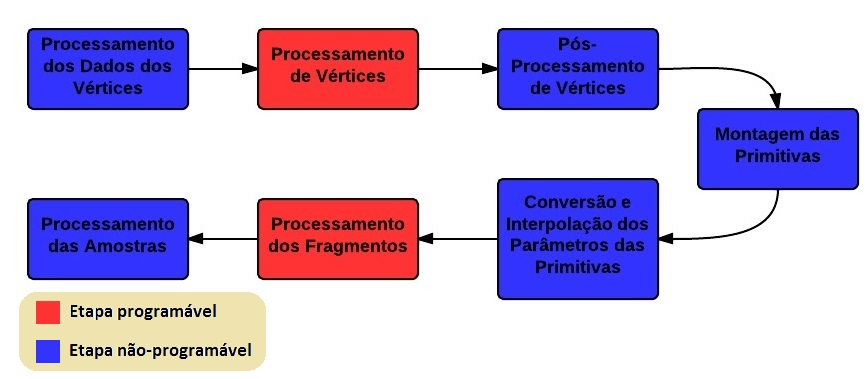
\includegraphics[keepaspectratio=true,scale=0.5]{figuras/pipeline.jpg}
	\caption{Processo de renderização da \textit{OpenGL}}
	\label{pipeline}
	\end{figure}

	 Assim, existem dois tipos de \textit{shader} principais, relacionados à criação de diferentes efeitos visuais, que focam partes distintas do \textit{pipeline} gráfico: o \textit{vertex shader} e o \textit{fragment shader}. O \textit{vertex shader} é responsável pela manipulação dos dados dos vértices, a partir das coordenadas de posição, normal e textura, por exemplo. Ele altera a etapa de processamento de vértices e deve, ao menos, definir as coordenadas de posição.  O \textit{fragment shader} opera na etapa de processamento dos fragmentos, e deve atribuir uma cor para cada fragmento.

\subsection{Linguagens dos \textit{shaders}}

	
	Os \textit{shaders} possuem uma linguagem de programação própria, que muitas vezes está vinculada com a API gráfica utilizada.  A Tabela \ref{lingshader} mostra as principais linguagens de programação de \textit{shaders} e as respectivas bibliotecas gráficas em que podem ser utilizadas. 

	\begin{table}[ht]
	\centering	
	\begin{tabularx}{0.9\textwidth}{lX}
		\toprule
		\textbf{Linguagem de Programação} & \textbf{Biblioteca Gráfica Suportada}  \\
		\midrule
		\textit{GLSL: OpenGL Shading Language} & \textit{OpenGL} \\
		\textit{HLSL: High Level Shading Language} & \textit{DirectX} e \textit{XNA} \\
		\textit{Cg: C for Graphics} & \textit{DirectX} e \textit{OpenGL}\\
		\bottomrule
	\end{tabularx}
	\caption{ Linguagens de programação para \textit{shaders}}
	\label{lingshader}
\end{table}

	A linguagem GLSL (\textit{OpenGL Shading Language}) foi incluída na versão 2.0 da  \textit{OpenGL}, sendo desenvolvida com o intuito de dar aos programadores o controle de partes do processo de renderização. A GLSL é baseada na linguagem C, mas antes de sua padronização o programador tinha que escrever o código na linguagem \textit{Assembly}, a fim de acessar os recursos da GPU. Além dos tipos clássicos do C, \textit{float}, \textit{int} e \textit{bool}, a GLSL possui outros tipos mostrados na Tabela \ref{tiposglsl}.

\begin{table}[ht]
	\centering	
	\begin{tabularx}{0.9\textwidth}{lX}
		\toprule
		\textbf{Tipo} & \textbf{Descrição}  \\
		\midrule
		\texttt{vec2}, \texttt{vec3}, \texttt{vec4} & Vetores do tipo \textit{float} de 2, 3 e 4 entradas \\
		\texttt{ivec2},\texttt{ivec3}, \texttt{ivec4} & Vetores do tipo inteiro de 2, 3 e 4 entradas \\
		\texttt{mat2}, \texttt{mat3}, \texttt{mat4} & Matrizes 2x2, 3x3 e 4x4 \\
		\texttt{sampler1D}, \texttt{sampler2D}, \texttt{sampler3D} & Acesso a texturas \\
		\bottomrule
	\end{tabularx}
	\caption{ GLSL: tipos de dados}
	\label{tiposglsl}
\end{table}

	Além disso, a GLSL possui variáveis chamadas qualificadoras, que fazem o interfaceamento do programa e os \textit{shaders} e entre \textit{shaders}. Algumas destas varáveis são mostradas na Tabela \ref{tiposqualificadores}.

	\begin{table}[ht]
	\centering	
	\begin{tabularx}{0.9\textwidth}{lX}
		\toprule
		\textbf{Tipo} & \textbf{Descrição}  \\
		\midrule
		\texttt{attribute} &  Variável utilizada pelo programa para comunicar dados relacionados aos vértices para o \textit{vertex shader}\\
		\texttt{uniform} &  Variável utilizada pelo programa para comunicar dados relacionados com as primitivas para ambos os \textit{shaders} \\
		\texttt{varying} &  Variável utilizada pelo \textit{vertex shader} para se comunicar com o \textit{fragment shader} \\
		\bottomrule
	\end{tabularx}
	\caption{ GLSL: qualificadores}
	\label{tiposqualificadores}
	\end{table}

\subsection{Utilização dos \textit{shaders} em \textit{OpenGL}}

	Para cada \textit{shader} -- relativos ao vértice e ao fragmento -- é necessário escrever o código que será compilado e feito o \textit{link}, gerando um programa final que será utilizado pela \textit{OpenGL}. Ou seja: é feita a compilação e o \textit{link} pela aplicacão de cada um destes\textit{shaders}. Caso os \textit{shaders} utilizem variáveis passadas pela \textit{OpenGL}, é necessário primeiramente encontrar a localização desta variável e depois setá-la. Se a variável for do tipo \textit{uniform}, por exemplo, adquire-se a localização por meio da função \texttt{glGetUniformLocation(GLuint program, const GLchar *name)}, em que \textit{program} é o programa gerado a partir dos \textit{shaders} e \textit{name} é o nome da variável definida dentro do \textit{shader}. 

	A Figura \ref{shader_use} mostra o processo de geração do programa a partir dos \textit{shaders} criados.

	\begin{figure}[ht]
	\centering
		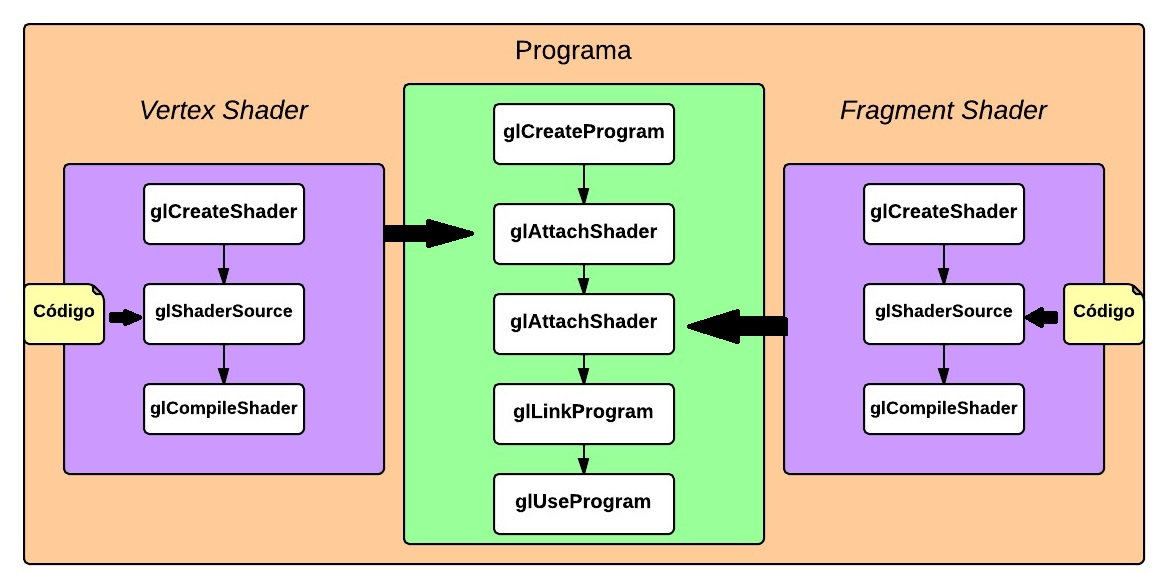
\includegraphics[keepaspectratio=true,scale=0.4]{figuras/shader_use.jpg}
	\caption{Utilização dos \textit{shaders}}
	\label{shader_use}
	\end{figure}


\subsection{\textit{Shaders} em Plataformas Móveis}

	Assim como para computadores, também existem bibliotecas gráficas para dispositivos móveis. Nas próximas seções são mostradas as plataformas \textit{Android} e \textit{iOS}, que foram utilizadas neste trabalho, e a biblioteca gráfica \textit{OpenGL ES}, que é uma variação da \textit{OpenGL} para dispositivos móveis, usada na programação de \textit{shaders}.

	\subsubsection{Plataforma \textit{Android}}

	O \textit{Android} começou a ser desenvolvido em 2003 na empresa de mesmo nome, fundada por Andy Rubin, a qual foi adquirida em 2005 pela empresa \textit{Google}. A \textit{Google} criou a \textit{Open Handset Alliance}, que une várias empresas da indústria das telecomunicações, como a \textit{Motorola} e a \textit{Samsung}, por exemplo. Assim, elas desenvolveram o \textit{Android} como é conhecido hoje, o qual é um sistema operacional  \textit{open source} para dispositivos móveis (baseado no \textit{kernel} do \textit{Linux}), tendo a primeira versão beta lançada em 2007 e segundo \cite{android2013}, hoje é o sistema operacional para \textit{mobile} mais utilizado. Em 2012, mais de 3,5 \textit{smartphones} com \textit{Android} eram enviados aos clientes para cada \textit{iPhone}. Em 2011, 500.000 novos \textit{devices} eram atividados a cada dia e em 2013, os números chegaram a 1,5 milhões diários. 

	O \textit{Android} também possui um mercado centralizado acessível por qualquer aparelho (\textit{tablet} ou \textit{smartphone}) chamado \textit{Google Play}\footnote{\textit{https://play.google.com/store}}, facilitando a publicação e aquisição de aplicativos. Ele também possui diferentes versões, sendo elas mostradas na Tabela \ref{androidTab}.  As versões mais novas possuem mais \textit{features} que as anteriores: a versão \textit{Jelly Bean}, por exemplo, possui busca por voz a qual não estava disponível na versão \textit{Ice Cream Sandwich}. 

\begin{table}[ht]
	\centering	
	\begin{tabular}{cl}
		\toprule
		\textbf{Número da versão} & \textbf{Nome}  \\
		\midrule
		1.5 &  \textit{Cupcake} \\
		1.6 & \textit{Donut} \\
		2.0/2.1 &  \textit{Éclair} \\
		2.2 & \textit{FroYo} \\
		2.3 &  \textit{Gingerbread} \\
		3.0/3.1/3.2 & \textit{HoneyComb} \\
		4.0 & \textit{Ice Cream Sandwich} \\
		4.1/4.2/4.3 & \textit{Jelly Bean} \\
		4.4 &  \textit{KitKat} \\

		\bottomrule
	\end{tabular}
	\caption{ Versões da plataforma \textit{Android}}
	\label{androidTab}
\end{table}


	\subsubsection{Plataforma \textit{iOS}}

	A plataforma \textit{iOS} é uma plataforma móvel que foi lançada em 2007 e é distribuída exclusivamente para \textit{hardware} frabricado pela \textit{Apple} (empresa que a desenvolveu).  De acordo com o CEO da \textit{Apple}, Tim Cook, mais de 800 milhões de aparelhos \textit{iOS} -- como o \textit{iPhone}, \textit{iPad} e \textit{iPod touch} -- já foram vendidos desde o seu lançamento. A plataforma \textit{iOS} é atualizada periodicamente (uma vez ao ano) e a Tabela \ref{iosv} mostra as versões de \textit{iOS} já lançadas.

	\begin{table}[ht]
	\centering	
	\begin{tabular}{cc}
		\toprule
		\textbf{Número da versão} & Ano Lançamento  \\
		\midrule
		iOS 1.x & 2007 \\
		iOS 2.x & 2008 \\
		iOS 3.x &  2009 \\
		iOS 4.x & 2010 \\
		iOS 5.x &  2011 \\
		iOS 6.x & 2012 \\
		iOS 7.x & 2013 \\
		iOS 8.x & 2014 \\	
		\bottomrule
	\end{tabular}
	\caption{ Versões da plataforma \textit{Android}}
	\label{iosv}
\end{table}

	Assim como a plataforma \textit{Android}, a \textit{iOS} também possui um mercado centralizado acessível por qualquer aparelho, chamado de \textit{Apple Store}\footnote{\textit{http://store.apple.com/br}}, para aquisição e publicação de aplicativos. 

	\subsubsection{\textit{OpenGL ES}}
	
	A \textit{OpenGL ES} (\textit{OpenGL for Embedded Systems}) foi lançada em 2003, sendo a versão da \textit{OpenGL} para sistemas embarcados, e como citado em \cite{guha2011}, atualmente é uma das API's mais populares para programação de gráficos tridimensionais em dispositivos móveis, sendo adotada por diversas plataformas como \textit{Android}, \textit{iOS}, Nintendo DS e \textit{Black Berry}.

	Segundo \cite{opengles2012}, ela possui três versões: a 1.x que utiliza as funções fixas de renderização, a 2.x, que elimina as funções fixas e foca nos processos de renderização manipulados por \textit{pipelines} programáveis (\textit{shaders}) e a 3.x, que é completamente compatível com a  \textit{OpenGL} 4.3.  

	A \textit{OpenGL ES}, assim como a \textit{OpenGL}, também utiliza a linguagem GLSL para programação de \textit{shaders} e  já faz parte das ferramentas de desenvolvimento da plataforma \textit{Android}. De acordo com \cite{buck2012}, na plataforma \textit{iOS} a \textit{OpenGL ES} pode ser utilizada por meio do \textit{framework} chamado \textit{GLKit} (introduzido no \textit{iOS} 5). Ele provê classes e funções que simplificam o uso da \textit{OpenGL ES} no contexto do \textit{iOS}.


\section{Fundamentação Matemática e Física para Implementação de \textit{Shaders}}
\label{teoria}

	Os efeitos visuais -- criados por meio dos \textit{shaders} -- são representações de descrições físicas, podendo atribuir materiais aos objetos e diferentes efeitos de luz, por exemplo. Assim, esta seção apresenta alguns conceitos necessários para o entendimento dos \textit{shaders} implementados.

	\subsection{Renderização \textit{Flat}, \textit{Gouraud} e \textit{Phong}}
	\label{flatgouphon}

	Na área de computação gráfica, {\textit{Flat Shading}, \textit{Gouraud Shading} e \textit{Phong Shading} são os \textit{shaders} mais conhecidos. No método \textit{Flat Shading}, renderiza-se cada polígono de um objeto com base no ângulo entre a normal da superfície e a direção da luz. Mesmo que as cores se diferenciem nos vértices de um mesmo polígono, somente uma cor é escolhida entre elas e é aplicada em todo o polígono.  

	A computação dos cálculos de luz nos  vértices seguida por uma interpolação linear dos resultados é denominada como \textit{Gouraud Shading} (considerada superior ao \textit{Flat Shading}, pois renderiza uma superfície mais suave, lisa), criada por Henri Gouraud, sendo conhecida como avaliação por vértice. Nela, o \textit{vertex shader} deve calcular a intensidade da luz em cada vértice e os resultados serão interpolados. Em seguida, o \textit{fragment shader} propaga este valor para as próximas etapas. 

	No \textit{Phong Shading}, primeiramente interpolam-se os valores das normais das primitivas e então computam-se os cálculos de luz para cada \textit{pixel}, utilizando as normais interpoladas. Este método também é conhecido como avaliação por \textit{pixel}. A intensidade da luz em um ponto da superfície, segundo \cite{guha2011}, é calculada de acordo com a Equação \ref{eqphong}.  

	\begin{equation}
		%I_ {total} = I_ {ambiente} +  \sum\limits_ {luzes} I_ {difusa} + I_ {especular}
	I_ {T} = I_ {A} +  \sum I_ {D} + I_ {E}
	\label{eqphong}
	\end{equation}
	onde $I_{T}$ é a iluminação total, $I_A$ é a iluminação ambiente, $I_D$ é a iluminação difusa e $I_E$ é a iluminação especular. 

	Assim, a intensidade de luz é calculada como a soma das intensidades ambiente, difusa (calculada para cada fonte de luz) e especular.  A intensidade de reflexão ambiente vem de todas as direções e quando atinge a superfície, espalha-se igualmente em todas as direções, sendo o seu valor constante. Ela pode ser calculada de acordo com a Equação \ref{eqamb}, onde $I_A$ é a intensidade de luz ambiende, $K_ {A}$ é o coeficiente de refletividade ambiente da superfície e $L_ {A}$ é a intensidade da componente ambiente da luz.

	\begin{equation}
		I_ {A} = K_ {A}L_ {A} 
	\label{eqamb}
	\end{equation}

	A intensidadede da reflexão difusa vem de uma direção e, assim como a ambiente, ao atingir uma superfície também espalha-se igualmente em todas as direções. Ela pode ser calculada de acordo com a Equação \ref{eqdif}, onde $I_D$ é a intensidade da reflexão difusa, $K_ {D}$ é o coeficiente de reflexão difusa da superfície, $L_ {D}$ é a intensidade da componente difusa da luz, $\vec{ l}$ é a fonte de luz, $\vec{ n}$ é o ponto em interesse.

	\begin{equation}
		I_ {D} = K_ {D}L_ {D}( \vec{ l} \cdot \vec{ n}) 
	\label{eqdif}
	\end{equation}

	 A luz especular vem de uma direção e reflete como um espelho, em que o ângulo de incidência é igual ao de reflexão, podendo ser calculada de acordo com a Equação \ref{eqesp}, onde $I_E$ é a intensidade da reflexão especular, $K_ {S}$ é o coeficiente de reflexão especular da superfície, $L_ {S}$ é a intensidade da componente especular da luz, $\vec{ r}$ é a direção da reflexão, $\vec{v}$ é o vetor de visão do ponto (observador) e $s$ é o expoente especular.

	\begin{equation}
		I_ {E} =K_ {S}L_ {S} (\vec{ r} \cdot \vec{ v})^s
	\label{eqesp}
	\end{equation}

	 O \textit{Phong Shading} requer maior poder de processamento do que a técnica \textit{Gouraud Shading}, pois cálculos nos vértices são computacionalmente menos intensos comparados aos cálculos feitos por \textit{pixels}. Porém, a desvantagem da técnica de \textit{Gouraud Shading} é que efeitos de luz que não afetam um vértice de uma superfície não surtirão efeito como, por exemplo, efeitos de luz localizados no meio de um polígono, os quais não serão renderizados corretamente. A Figura \ref{fgp} mostra a diferença entre as três técnicas de \textit{shading} aplicadas em uma esfera com uma luz direcional. 

	\begin{figure}[ht]
	\centering
		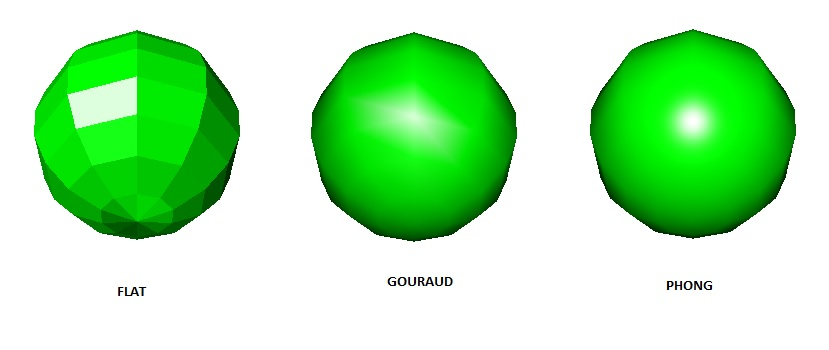
\includegraphics[keepaspectratio=true,scale=0.5]{figuras/flatgp.jpg}
	\caption{Comparação entre as técnicas de \textit{shading}}
	\label{fgp}
	\end{figure}

	\subsection{Renderização de Efeito \textit{Cartoon}}
	\label{cartoon}

	A renderização de efeito \textit{cartoon} tem como objetivo emular o efeito de um desenho, que tem como principal característica a aparência uniforme das cores sobre a superfície dos objetos. Isto pode ser feito mapeando-se faixas de intensidade de luz para tons de cores específicos, obtendo-se uma iluminação menos realista e mais próxima da utilizada em desenhos animados. De acordo com \cite{sbgames}, o tom é escolhido baseado no cosseno do ângulo entre a direção da luz e o vetor normal da superfície. Ou seja, se o vetor normal está mais próximo da direção da luz, utiliza-se um tom mais claro.  Então a intensidade da luz pode ser calculada de acordo com a Equação \ref{eqtoon}, onde $I_L$ é a intensidaded a luz, $\vec{l_{d}}$ é o vetor da direção da luz e $\vec{n}$ é o vetor normal.

	\begin{equation}
		I_ {L} = \frac{ \vec{l_{d}} \cdot \vec{n} } {\Vert \vec{l_{d}} \Vert  \Vert \vec{n} \Vert } 
	\label{eqtoon}
	\end{equation}

	Como os vetores $\vec{l_{d}}$ e $\vec{n}$ são normalizados, o cálculo pode ser simplificado de acordo com a Equação \ref{eqtoons}.

	\begin{equation}
		I_ {L} =  \vec{l_{d}} \cdot \vec{n}  
	\label{eqtoons}
	\end{equation}

	Após o cálculo da intensidade da luz, ela é mapeada para os tons pré-definidos, como mostra a Figura \ref{tons}.

	\begin{figure}[ht]
	\centering
		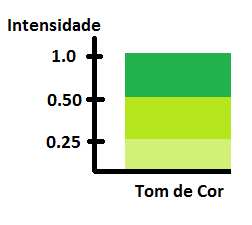
\includegraphics[keepaspectratio=true,scale=1.0]{figuras/tomcor.png}
	\caption{Exemplo de escolha dos tons}
	\label{tons}
	\end{figure}

	\subsection{Renderização de Efeito de Reflexão}
	\label{ref_t}

	O efeito de reflexão é obtido através da utilização da técnica chamada \textit{environment mapping}, na qual se reflete uma textura, que é desenhada ao redor do objeto e representa o cenário, chamada de \textit{environment map}. Um exemplo de textura utilizada por esta técnica é apresentada na Figura \ref{environment}.

	\begin{figure}[ht]
	\centering
		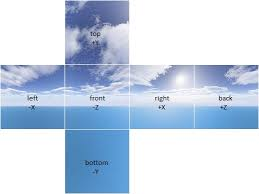
\includegraphics[keepaspectratio=true,scale=1.0]{figuras/envmap.jpg}
	\caption{\textit{Environment Map}}
	\label{environment}
	\end{figure}

	Assim, a ideia é obter um vetor que vai da posição da câmera ao objeto e refletí-lo, baseando-se na normal da superfície. Isto gera um outro vetor que é utilizado para determinar a cor, baseando-se na textura (\textit{environment map}).

\section{Complexidade Assintótica}
\label{metminquad}

	Complexidade assintótica é uma medida que compara a eficiência de um determinado algoritmo, analisando o quão custoso ele é (em termos de tempo, memória, custo ou processamento). Ela foi desenvolvida por Juris Hartmanis e Richard E. Stearns no ano de 1965. Segundo \cite{complexidade}, para não depender do sistema em que está sendo rodado e nem da linguagem de programação, a complexidade assintótica se baseia em uma função (medida lógica) que expressa uma relação entre a quantidade de dados e de tempo necessário para processá-los. Assim, é possível calcular a complexidade assintótica de um código de forma teórica e experimental.

	\subsection{Abordagem Teórica}

	 O cálculo da complexidade assintótica visa a modelagem do comportamento do desempenho do algoritmo, a medida que o número de dados aumenta. Assim, os termos que não afetam a ordem de magnitude são eliminados, gerando a aproximação denominada complexidade assintótica. Assim, a  Equação (\ref{compl1})

	\begin{equation}
		y = n^{2} +10 n + 1000
	\label{compl1}
	\end{equation}
 poderia ser aproximada pela  Equação (\ref{compl2}).


	\begin{equation}
		y \approx  n^{2} 
	\label{compl2}
	\end{equation}

	A maioria dos algoritmos possui um parâmetro $n$ (o número de dados a serem processados), que afeta mais significativamente o tempo de execução. De acordo com \cite{complexidade2}, a maioria dos algorítmos se enquadram nos tempos de execução proporcionais aos valores da Tabela \ref{complexidadeAlgoritmica}. A Figura \ref{compalg} mostra uma comparação entre estas curvas. 

\begin{table}[ht]
	\centering	
	\begin{tabularx}{0.9\textwidth}{cX}
		\toprule
		\textbf{Complexidade} & \textbf{Descrição}  \\
		\midrule
		Constante &  Ocorre quando as instruções do programa independem do número de elementos de entrada.\\
		log N & Ocorre geralmente em programas que resolvem grandes problemas dividindo-os em partes menores, reduzindo o seu tamanho por uma razão constante.  \\
		N & Ocorre quando o programa é linear, ou seja, o  processamento é feito para cada elemento de entrada. \\
		$ N log N$ & Ocorre quando o problema é quebrado em partes menores, sendo resolvidas independentemente, e depois suas soluções são combinadas. \\
		$ N^{2}$ & Ocorre quando o algoritmo é quadrático, ou seja, quando processa todos os pares da entrada. \\
		$ N^{3}$ & Ocorre quando o algoritmo é cúbico, ou seja, quando processa todos as triplas da entrada. \\
		$ 2^{N}$ & Ocorre quando o algoritmo segue uma função exponencial, ou seja, quando o N dobra o tempo de execução é elevado ao quadrado. \\
	
		\bottomrule
	\end{tabularx}
	\caption{ Valores mais comuns de complexidade assintótica}
	\label{complexidadeAlgoritmica}
\end{table}


	\begin{figure}[ht]
	\centering
		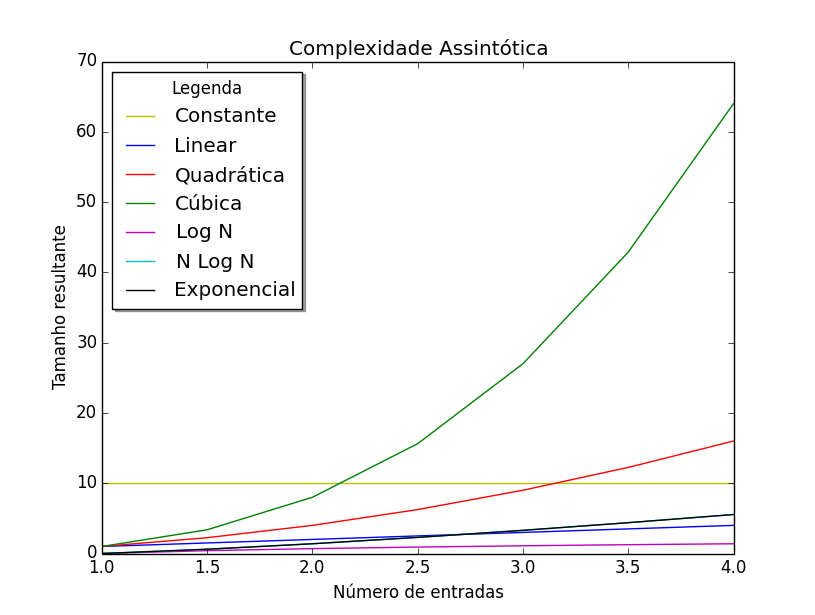
\includegraphics[keepaspectratio=true,scale=0.4]{figuras/compalg.png}
	\caption{Comparação da Complexidade Assintótica}
	\label{compalg}
	\end{figure}

	\subsubsection{Notação \textit{Big-O}}

	
	A notação \textit{Big-O} foi desenvolvida em 1894 por Paul Bachmann para complexidade assintótica. Assim, segundo \cite{complexidade}, dadas duas funções de valores positivos $f$ e $g$, $f(n)$ é $O(g(n))$ se existem $c$ e $N$ positivos tais que $f(n) \leq cg(n)$, $\forall n \geq N$. Ou seja, dada uma função $g(n)$, denota-se por $O(g(n))$ o conjunto das funções que para valores de $n$ suficientemente grandes, $f(n)$ é igual ou menor que $g(n)$. A função $f$ tende a crescer no máximo tão rápido quanto $g$, em que $cg(n)$ é uma cota superior de $f(n)$. O algorítmo $y = n^{2} +10 n + 1000$, por exemplo, é $O(n^2)$. 

	Se $f(n)$ é um polinômio de grau $d$  então $f(n)$ é $O(n^d)$. E como uma constante pode ser considerada de grau zero, sua complexidade é $O(n^0)$, ou seja, $O(1)$. Além disso, a função $f(n) = \log _a \left( n \right)$ é $O(\log _b \left( n \right))$ para quaisquer $a$ e $b$ positivos diferentes de 1. 

	\subsection{Abordagem Experimental}
	\label{metminqua}

	Como não é possível determinar a complexidade assintótica dos \textit{shaders} de forma teórica, pois não estão disponíveis as implementações das funções da API da GLSL, uma das formas de calculá-la é de maneira experimental. Isto é feito variando o número de entradas e coletando uma medição associada ao desempenho, como o tempo, por exemplo. Assim, é possível gerar um gráfico e utilizar o método dos mínimos quadrados para descobrir qual curva melhor aproxima estes pontos. O método dos mínimos quadrados é usado para ajustar um conjunto de pontos $(x,y)$ a uma determinada curva. 

	\subsubsection{Ajuste Linear}

	No caso do ajuste à uma reta (dada por $y = a + bx$), por exemplo, muitas vezes os pontos não são colineares e segundo \cite{minq} é impossível encontrar coeficientes $a$ e $b$ que satisfaçam o sistema.  Então, as distâncias destes valores para a reta podem ser consideradas como medidas de erro e os pontos são minimizados pelo mesmo vetor (minimizando a soma dos quadrados destes erros).  Assim, existe um ajuste linear de erros mínimos quadrados aos dados, e a sua solução é dada pela Equação (\ref{minquad}), em que é possível determinar os coeficientes $a$ e $b$ e, consequentemente, a equação da reta que constitui a aproximação. 

	\begin{equation}
		v =( M^{T}M)^{-1}M^{T}y
	\label{minquad}
	\end{equation}
	onde
	\begin{equation}
	M = \left[\begin{array}{cc}
               	1 & x_{1} \\
               	1 & x_{2}  \\
		\vdots & \vdots  \\
		1 & x_{n}
          	         \end{array}\right] \mbox{,} \quad
	v = \left[\begin{array}{c}
               	a \\
               	b  
          	         \end{array}\right] \mbox{e} \quad
	y = \left[\begin{array}{c}
               	y_{1} \\
               	y_{2}  \\
	 \vdots  \\
		y_{n}
          	         \end{array}\right] 	
	\label{variaveis}
	\end{equation}

	\subsubsection{Ajuste Exponencial}

	De acordo com \cite{calculo}, a função da exponencial pode ser dada como na Equação (\ref{expo}), em que $e$, $c$, $k$ são constantes ($e$ é a constante neperiana).  

	\begin{equation}
	\label{expo}
		y = ce^{-kt}
	\end{equation}

	Aplicando a função logarítimo dos dois lados da equação, obtém-se a  Equação (\ref{expo2})

	\begin{equation}
	\label{expo2}
		\ln{y} = \ln{c}  + \ln{e^{-kt}}
	\end{equation}
 	que pode ser simplificada na  Equação (\ref{eqn03}) (onde $\bar{b}$ é uma nova constante) que equivale à equação da reta. 

	\begin{equation}
	\label{eqn03}
		\bar{y} = \bar{a} + \bar{b}t
	\end{equation}	

	Assim, é possível aplicar o método dos mínimos quadrados descrito anteriormente, aplicando o logaritmo nos dois lados da equação da exponencial. Os novos valores de $M$ e $y$ passam a ser: 

	\begin{equation}
	M = \left[\begin{array}{cc}
               	1 &  x_{1} \\
               	1 & x_{2}  \\
		\vdots & \vdots  \\
		1 & x_{n}
          	         \end{array}\right] \mbox{,} \quad
	y = \left[\begin{array}{c}
               	\ln{y_{1}} \\
               	\ln{y_{2}}  \\
		\vdots \\
		\ln{y_{n}}
          	         \end{array}\right] 
	\label{nvar}
	\end{equation}

	O valores finais dos coeficientes $\bar{a}$ e $\bar{b}$ determinam os parâmetros $c$ e $k$ da exponecial através das relações

	\begin{equation}
	c = e^{\bar{a}}\, \, \, \mbox{e}\, \, \,\bar{b} = -k
	\end{equation} 

	\subsubsection{Ajuste para Polinômio de Segundo e Terceiro Grau}

	O ajuste de segundo grau é parecido com o linear, em que a Equação \ref{minquad} também é utilizada. Porém a matriz M é redefinida para:

	\begin{equation}
	M = \left[\begin{array}{ccc}
               	1 & x_{1} & x_{1}^{2} \\
               	1 & x_{2}  & x_{2}^{2}\\
		\vdots & \vdots & \vdots \\
		1 & x_{n} & x_{n}^{2}
          	         \end{array}\right] \quad
	\label{minquadsegdeg}
	\end{equation}


	O ajuste de terceiro grau ocorre da mesma forma que o de segundo grau, mas a matriz M é redefinida para:

	\begin{equation}
	M = \left[\begin{array}{cccc}
               	1 & x_{1} & x_{1}^{2} & x_{1}^{3} \\
               	1 & x_{2}  & x_{2}^{2} & x_{1}^{3}\\
		\vdots & \vdots  & \vdots & \vdots\\
		1 & x_{n} &  x_{n}^{2} & x_{n}^{3}
          	         \end{array}\right] \quad
	\label{minquathirddeg}
	\end{equation}

	\subsubsection{Cálculo dos Erros dos Ajustes}

	O cálculo dos erros dos ajustes para as funções é calculado a fim de saber qual delas melhor se aproxima ao conjunto de pontos. Estes erros são calculados de acordo com a Equação \ref{erros}, em que cada erro ($e_{n}$) está associado à distância do ponto gerado pela curva ajustada e o ponto original.

	\begin{equation}
	E = \sqrt[2]{e_{1} + e_{2} + \dots + e_{n}}
	\label{erros}
	\end{equation} 


